% Ziele: Story hooks
% Mehr Drama als eine Telenovella
% Man muss zig Abenteuer aus der Konstellation ziehen können
% Die Meisten Charaktere sind ü 60 und haben viel erlebt. Das aufzählen.

\chapter{The Lost flea market}

There are many Lost flea markets. This one is mobile. It travels around the country, creating a meeting point for different Lost groups. However, some Norms and Pioneers are also attracted to it and are left confused.

A radio message notifies the Lost community when a flea market is taking place in their area. It's an important event. However, organising these markets requires a great deal of effort. By a very special kind of people.

These people will be introduced here.

\section{If it succeeds....}

If the flea market is successful this time, it will be a mixture of smells, including food, unplugged music, trade and barter, theatre, and the noise of blacksmiths and animals. Different dialects mingle. It is a giant, low-tech festival where normally hostile groups meet.

Friendships are formed. Plans are made and goods, stories and rumours are traded.

At night, torches and campfires light it up. People chat, sing and tell stories late into the night. People drink, smoke and eat together.

After about two weeks, all 500 people have left.

Great things can happen in those two weeks:

\subsection{Random events}

\begin{enumerate}
    \item Old Jacob wants to share his famous bathtub gin recipe before he dies. He will reveal this secret to the first three people to bring him a special alcoholic beverage.
    \item At night there is a spontaneous fire-juggling show
    \item Someone is running a quiz 'The 1980se'. You can win a bottle of Jacob's bathtub-gin.
    \item Two people are getting engaged. To celebrate, a whole pig is being barbecued. Norms and pioneers alike may experience culture shock.
    \item There is a Shakespeare competition. Two groups are competing, but they still need actors for some roles.
    \item Both adults and children over the age of 14 can learn to shoot a semi-automatic weapon at the shooting range. This may confuse some Norms.
\end{enumerate}


\chapter{The task}

The flea market team travels around, announcing the event on the radio and preparing for around 500 people. Most of those Lost will contribute to the flea market. They will contribute by selling food, running craft stalls and so on.

The flea market team provides the base infrastructure. They also try to connect hostile Lost groups. This is one of the reasons for creating a flea market (others include trade, knowledge and entertainment).

Player characters could arrive while the flea market is being set up. They could help out and make new friends. After two weeks, everyone will move on.

\section{The problems}

Building a flea market is never straightforward. Expect problems. Thankfully, NPCs, the protagonists and perhaps some early arrivals will solve them.

\subsection{Random events during set up}

\begin{enumerate}
\item A guest group arrives too late - what could have happened ?
\item A guest group arrives too early
\item The field where the planned flea market is to be held is flooded after heavy rain. It has turned into a lake. It is full of stinging nettles and scrub.
\item A buried Lemming ruin has been found where the flea market is due to be built. The Jones-es want to loot it. This could lead to a dungeon crawl.
\item The creation of the flea market is slowing down. Everyone is distracted by the tasty food.
\item Curious children from the nearby Pioneer camp come to visit in their exoskeletons. Lost are caught between feeling scared and protective because of the technology.
\end{enumerate}

\section{Wendy and family}

The plot of the NPCs Wendy and her family is akin to a telenovela drama. If you don't want this kind of plot, remove or modify it.

\chapter{The NPCs}

\section{Animal expert: Jonas Ohnesorg}

He organises shelter for animals ranging from rabbits to cattle. In doing so, he also ensures the health of the bartered animals and the supply of feed. He also runs a local butcher's shop. When he is not organising the flea market, he is a trainer for birds of prey. However, sometimes these birds catch rabbits, including those owned by farmers.

\begin{center}
    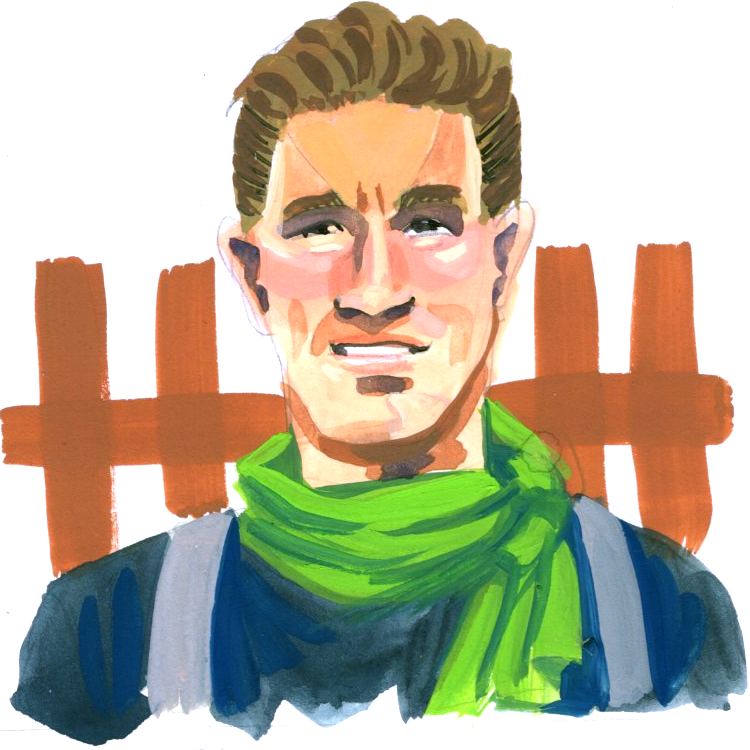
\includegraphics[scale=0.4]{portraits/Flohmarkt_Jonas.png}
\end{center}

\newpage
\begin{npcBox}[title=Jonas Ohnesorg]

    \begin{aspects}
    \item \aspect[High Concept]{He loves animals more than they love him}
    \item \aspect[Trouble]{Others are always tempted to handle his animals without care}
    \item \aspect[Relationship]{Loves Antigone}
    \item \aspect[Aspect]{He loves eating hot food — he needs a kick in his life!}
    \end{aspects}

    \begin{skills}
    \item \nskill{Academics}{0}
    \item \nskill{Athletics}{1}
    \item \nskill{Burglary}{0}
    \item \nskill{Contacts}{1}
    \item \nskill{Crafts}{3}
    \item \nskill{Deceive}{0}
    \item \nskill{Drive}{0}
    \item \nskill{Empathy}{1}
    \item \nskill{Fight}{3}
    \item \nskill{Investigate}{0}
    \item \nskill{Lore}{0}
    \item \nskill{Notice}{1}
    \item \nskill{Physique}{2}
    \item \nskill{Provoke}{0}
    \item \nskill{Rapport}{2}
    \item \nskill{Resources}{0}
    \item \nskill{Shoot}{0}
    \item \nskill{Stealth}{0}
    \item \nskill{Will}{2}
    \item \nskill{Bushcraft}{4}
    \end{skills}

    \begin{stunts}
    \item \stunt{Animal whisperer}{Gets +2 on Bushcraft when teaching and commanding animals.}
    \end{stunts}

    \begin{stressSection}
    \stressLine{\stress{1}\stress{1}\stress{1}\stress{1}}{\stress{1}\stress{1}\stress{1}\stress{1}}
    \end{stressSection}
    \begin{tabularx}{\textwidth}{ XX }
    \end{tabularx}

    \begin{consequences}
    \item \consequence{2}
    \item \consequence{4}
    \item \consequence{6}
    \end{consequences}

    \begin{equipment}
    \item His eagle "Igel" (Hedgehog in German). He still thinks this is funny.
    \item Equipment for the different animals.
    \end{equipment}
\end{npcBox}


\subsection{Random events involving animals}

\begin{enumerate}
\item An animal escapes
\item An animal is ill. There is a risk of an outbreak - can someone find a vet ?
\item Animals give birth to their young
\item The animals confuse the Norms and Pioneers. They want to pet them, keep them or film them, which often turns into a disaster.
\item The animals are starving. Someone must get a truckload of food.
\item His birds of prey start hunting small animals
\end{enumerate}

\newpage
\section{Kitchen and military tactics: Gustav Müller}

His core theses: order, discipline and sauces are central

Favourite silly saying: 'No food, no fight'

There is little difference between managing a kitchen and organising a battle. For him, both involve leading small units. His attitude leads him to defend the Lost Camp or to set up a large kitchen for a flea market. His imperious military manner may bring him success, but it also makes him enemies.

Info for GM: This is how commercial kitchens really came about. From military structures: \href{https://en.wikipedia.org/wiki/Kitchen_brigade}{Kitchen brigade}

\begin{center}
    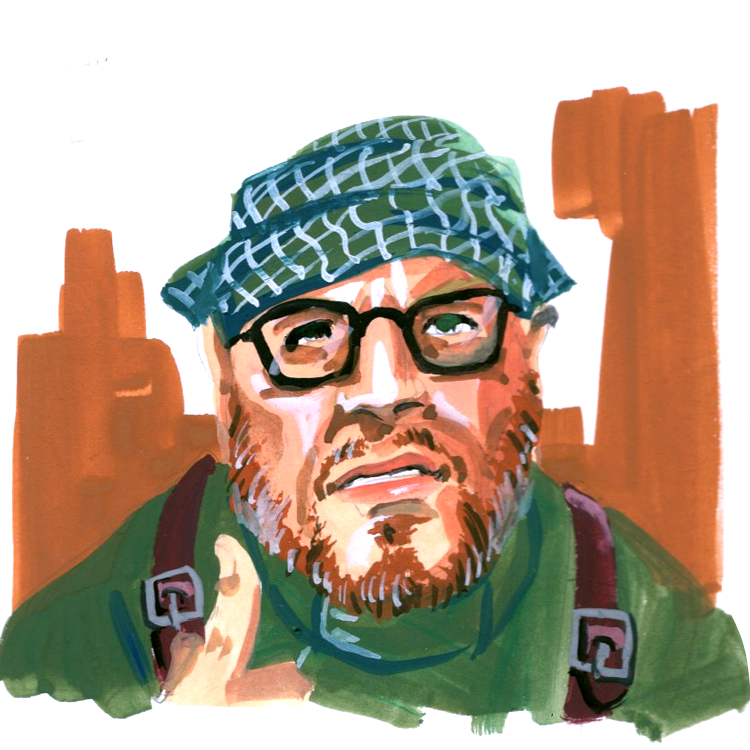
\includegraphics[scale=0.4]{portraits/Flohmarkt_Gustav.png}
\end{center}

\newpage
\begin{npcBox}[title=Gustav Müller]

    \begin{aspects}
    \item \aspect[High Concept]{Perfectly organized kitchen general}
    \item \aspect[Trouble]{Hard to himself - 'till he drops}
    \item \aspect[Relationship]{He does not have any closer relationsships to other humans}
    \item \aspect[Aspect]{Perfection is in the details - and beautiful ornaments}
    \end{aspects}

    \begin{skills}
    \item \nskill{Academics}{0}
    \item \nskill{Athletics}{1}
    \item \nskill{Burglary}{0}
    \item \nskill{Contacts}{0}
    \item \nskill{Crafts - Cooking}{3}
    \item \nskill{Deceive}{0}
    \item \nskill{Drive}{1}
    \item \nskill{Empathy}{0}
    \item \nskill{Fight}{1}
    \item \nskill{Investigate}{0}
    \item \nskill{Lore}{2}
    \item \nskill{Notice}{1}
    \item \nskill{Physique}{2}
    \item \nskill{Provoke}{2}
    \item \nskill{Rapport}{0}
    \item \nskill{Resources}{0}
    \item \nskill{Shoot}{3}
    \item \nskill{Stealth}{0}
    \item \nskill{Will}{4}
    \end{skills}

    \begin{stunts}
    \item \stunt{Structured}{He gets +2 on Craft and shooting if there is a clear hierarchy. -2 if the org chart is chaotic.}
    \end{stunts}

    \begin{stressSection}
    \stressLine{\stress{1}\stress{1}\stress{1}\stress{1}}{\stress{1}\stress{1}\stress{1}\stress{1}\stress{1}\stress{1}}
    \end{stressSection}
    \begin{tabularx}{\textwidth}{ XX }
    \end{tabularx}

    \begin{consequences}
    \item \consequence{2}
    \item \consequence{4}
    \item \consequence{6}
    \end{consequences}

    \begin{equipment}
    \item GLarge cooking appliances. Entire trailers converted into kitchen units.
    \item A Desert Eagle
    \end{equipment}
\end{npcBox}


\subsection{Random events}

\begin{enumerate}
\item He has a truck containing an herb garden. Currently, it is not close to the kitchen tents. Someone forgot that. Now someone has to drive it through the flea market to get it there.
\item Someone needs to improvise a giant mixer using a diesel generator and some equipment.
\item A long table is set up through the entire flea market and everyone is invited to a banquet - if it works!
\item Gustav leaves the kitchen in the hands of his sous chef for a few hours. He has to attend combat tactics exercises in the nearby forest.
\item He has been asked if he can provide shooting training for children and adults. He can do so if he receives assistance with the kitchen and construction of the shooting range.
\item People are being rudely thrown out of the kitchen. There's trouble.
\end{enumerate}

\newpage

\section{Funk: Antigone Freitag}

She knows everyone on the radio waves and speaks many languages. Her goal is to complete her collection of Lemmings figurines. To this end, she regularly checks in with her radio contacts, and she has even sent out a rescue team to retrieve one of the missing figurines. Unfortunately, she cannot go herself as she is wheelchair-bound. However, the whole world comes to her via radio.

\begin{center}
    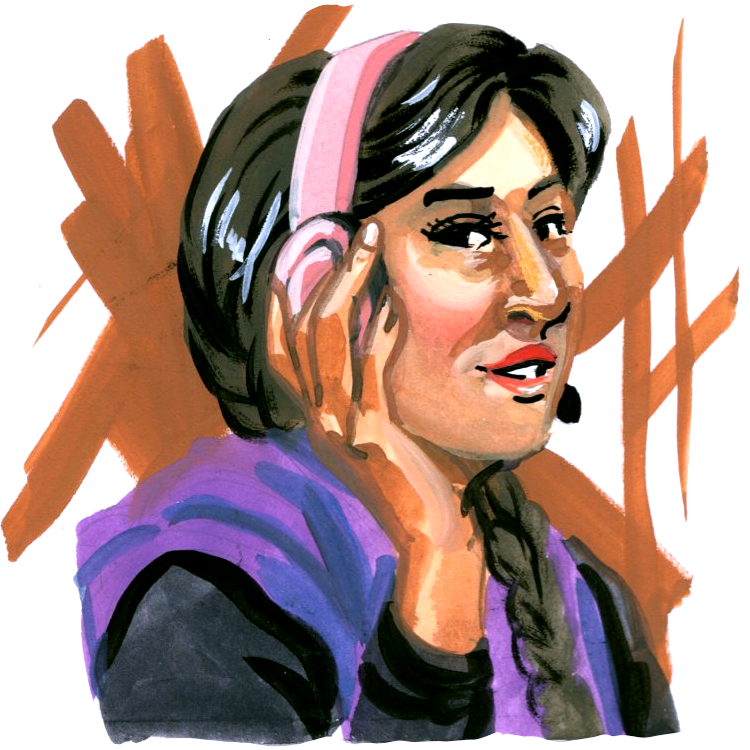
\includegraphics[scale=0.4]{portraits/Flohmarkt_Antigone.png}
\end{center}

\newpage
\begin{npcBox}[title=Antigone]

    \begin{aspects}
    \item \aspect[High Concept]{Radio operator and social encyclopaedia}
    \item \aspect[Trouble]{Knows almost everyone closely - but often has no idea what people look like.}
    \item \aspect[Relationship]{Because she knows everyone very well, she doesn't have anyone special.}
    \item \aspect[Aspect]{My trained little dog makes me more flexible and mobile.}
    \end{aspects}

    \begin{skills}
    \item \nskill{Academics}{3}
    \item \nskill{Athletics}{1}
    \item \nskill{Burglary}{0}
    \item \nskill{Contacts}{3}
    \item \nskill{Crafts - Radio}{2}
    \item \nskill{Deceive}{0}
    \item \nskill{Drive}{0}
    \item \nskill{Empathy}{2}
    \item \nskill{Fight}{0}
    \item \nskill{Investigate}{1}
    \item \nskill{Lore}{1}
    \item \nskill{Notice}{2}
    \item \nskill{Physique}{0}
    \item \nskill{Provoke}{0}
    \item \nskill{Rapport}{4}
    \item \nskill{Resources}{0}
    \item \nskill{Shoot}{0}
    \item \nskill{Stealth}{0}
    \item \nskill{Will}{1}
    \end{skills}

    \begin{stunts}
    \item \stunt{Seeing with my ears}{She is so accustomed to radio contact that she gets a +2 to empathy with her eyes closed, just by listening.}
    \end{stunts}

    \begin{stressSection}
    \stressLine{\stress{1}\stress{1}\stress{1}}{\stress{1}\stress{1}\stress{1}\stress{1}}
    \end{stressSection}
    \begin{tabularx}{\textwidth}{ XX }
    \end{tabularx}

    \begin{consequences}
    \item \consequence{2}
    \item \consequence{4}
    \item \consequence{6}
    \end{consequences}

    \begin{equipment}
    \item Her little mixed-breed dog “Snack”, who can fetch things on command.
    \item Radio equipment
    \item Soldering station
    \end{equipment}
\end{npcBox}

\subsection{Random events}

\begin{enumerate}
\item She found someone on the radio who has collectible figures. And that person is at the flea market. Since there is no radio contact, the protagonists have to find the person based on the description.
\item An arriving group is in danger and the PCs must guide them here.
\item Radio repeaters must be built and distributed to groups that will be leaving soon.
\item The radio fails. An amplifier and electronics are quickly needed from the flea market.
\item She wants to travel through the flea market too. But her wheelchair is impractical in the mud. She needs help. On the trip, she will see many of the people she usually only talks to for the first time.
\item She wants to broadcast a flea market radio programme. Receivers need to be distributed and content created.
\end{enumerate}

\newpage

\section{Gaia priest Laura}

Laura is a Gaianist. She is an inexperienced priestess in a newly established religion. Living in isolation, she is very grateful for any spiritual input, such as books or conversations. She often tries to explain Gaia to others, but quickly becomes flustered when things become more complex.

\begin{center}
    
\includegraphics[scale=0.4]{portraits/Flohmarkt_Laura.png}
\end{center}

\newpage
\begin{npcBox}[title=Laura, Gaianistin]

    \begin{aspects}
    \item \aspect[High Concept]{Inexperienced Gaianist}
    \item \aspect[Trouble]{The shoes are too big.}
    \item \aspect[Relationship]{She just joined the flea market - and does not know many people there}
    \item \aspect[Aspect]{Just found the way, highly enthusiastic and still stumbling}
    \end{aspects}

    \begin{skills}
    \item \nskill{Academics}{3}
    \item \nskill{Athletics}{1}
    \item \nskill{Burglary}{0}
    \item \nskill{Contacts}{1}
    \item \nskill{Crafts}{0}
    \item \nskill{Deceive}{0}
    \item \nskill{Drive}{0}
    \item \nskill{Empathy}{3}
    \item \nskill{Fight}{0}
    \item \nskill{Investigate}{2}
    \item \nskill{Lore}{2}
    \item \nskill{Notice}{1}
    \item \nskill{Physique}{0}
    \item \nskill{Provoke}{0}
    \item \nskill{Rapport}{4}
    \item \nskill{Resources}{1}
    \item \nskill{Shoot}{0}
    \item \nskill{Stealth}{0}
    \item \nskill{Will}{2}
    \end{skills}

    \begin{stunts}
    \item \stunt{Mandala}{With the right materials and time, she can lay an inspiring mandala that gives attentive observers +2 to Willpower. Even with care, the mandala lasts a maximum of 2 days.}
    \end{stunts}

    \begin{stressSection}
    \stressLine{\stress{1}\stress{1}\stress{1}}{\stress{1}\stress{1}\stress{1}\stress{1}}
    \end{stressSection}
    \begin{tabularx}{\textwidth}{ XX }
    \end{tabularx}

    \begin{consequences}
    \item \consequence{2}
    \item \consequence{4}
    \item \consequence{6}
    \end{consequences}

    \begin{equipment}
    \item Tea herbs - fresh and dried ones
    \item A tea tent
    \end{equipment}
\end{npcBox}


Gaia priests have dedicated themselves to Gaia, the living Earth. They strive for unity between the eco-, techno- and sociospheres. They particularly try to encourage others to build bridges. For example, they encourage collaboration between hostile groups and the implementation of joint projects.

\newpage


\section{Heavy machines: Wendy}

Head of logistics, heavy machinery and truck driver: Wendy (formerly Wilhelm). Her marriage to Doris broke down before the disaster. She didn't know why. Later, she realised that she was transgender and therefore a woman. She has a photo from the old days behind her sun visor. It shows him with Doris, his wife. Before the disasters, they used to travel through Europe in their truck. The marriage failed because Wilhelm/Wendy was always on the road and Doris was more settled. They have one child, “Flash”. The Lost don't know that Wendy used to be Wilhelm.

\begin{center}
    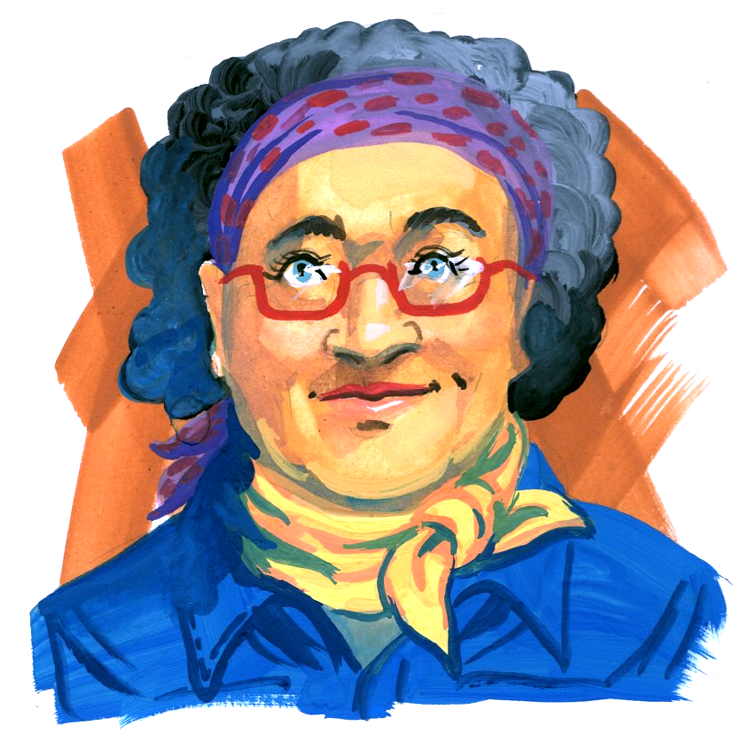
\includegraphics[scale=0.4]{portraits/Flohmarkt_Wendy.png}
\end{center}

\newpage
\begin{npcBox}[title=Wendy]

    \begin{aspects}
    \item \aspect[High Concept]{Heavy machines make me happy}
    \item \aspect[Trouble]{At home on the road}
    \item \aspect[Relationship]{Failed marriage to Doris because Doris is too settled.}
    \item \aspect[Aspect]{Daily exercise is necessary for my mental health.}
    \end{aspects}

    \begin{skills}
    \item \nskill{Academics}{0}
    \item \nskill{Athletics}{1}
    \item \nskill{Burglary}{0}
    \item \nskill{Contacts}{0}
    \item \nskill{Crafts}{3}
    \item \nskill{Deceive}{0}
    \item \nskill{Drive}{4}
    \item \nskill{Empathy}{2}
    \item \nskill{Fight}{0}
    \item \nskill{Investigate}{0}
    \item \nskill{Lore}{0}
    \item \nskill{Notice}{2}
    \item \nskill{Physique}{3}
    \item \nskill{Provoke}{1}
    \item \nskill{Rapport}{1}
    \item \nskill{Resources}{0}
    \item \nskill{Shoot}{0}
    \item \nskill{Stealth}{0}
    \item \nskill{Will}{2}
    \item \nskill{Bushcraft}{1}
    \end{skills}

    \begin{stunts}
    \item \stunt{Heavy weight}{Wendy gets +2 on driving if the vehicle weights mor than 5 tons}
    \end{stunts}

    \begin{stressSection}
    \stressLine{\stress{1}\stress{1}\stress{1}\stress{1}\stress{1}\stress{1}}{\stress{1}\stress{1}\stress{1}\stress{1}}
    \end{stressSection}
    \begin{tabularx}{\textwidth}{ XX }
    \end{tabularx}

    \begin{consequences}
    \item \consequence{2}
    \item \consequence{4}
    \item \consequence{6}
    \end{consequences}

    \begin{equipment}
    \item Access to excavators, lorries and forklifts belonging to the flea market organisation
    \item A set of heavy weights for her training
    \item A makeup set
    \end{equipment}
\end{npcBox}
\newpage

\section{Norm documentarian Doris}

She is on an adventure trip (without sanitary facilities, artificial meat, drones or networking): She used to be married to Wilhelm. She still carries the ring in her pocket, but doesn't know that his name is Wendy now. Will they get back together?
She is going on the adventure trip because she made a bet with her friends. Her friends know that her ex is somewhere among the lost and hope that they will get back together. Doris has often told them about their time together.

\begin{center}
    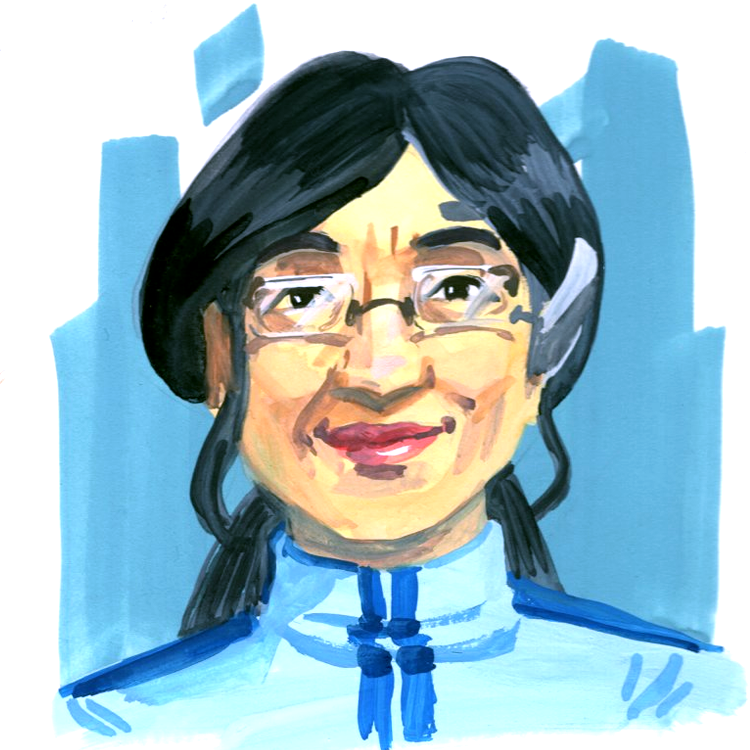
\includegraphics[scale=0.4]{portraits/Flohmarkt_Doris.png}
\end{center}

\newpage
\begin{npcBox}[title=Doris]

    \begin{aspects}
    \item \aspect[High Concept]{City spoiled - and looking for an adventure}
    \item \aspect[Trouble]{Searching for her lost past}
    \item \aspect[Relationship]{Her friends know better than she does who she is missing.}
    \item \aspect[Aspect]{Settled - with strong connections}
    \end{aspects}

    \begin{skills}
    \item \nskill{Academics}{3}
    \item \nskill{Athletics}{0}
    \item \nskill{Burglary}{0}
    \item \nskill{Contacts}{1}
    \item \nskill{Crafts}{0}
    \item \nskill{Deceive}{0}
    \item \nskill{Drive}{0}
    \item \nskill{Empathy}{3}
    \item \nskill{Fight}{0}
    \item \nskill{Investigate}{1}
    \item \nskill{Lore}{0}
    \item \nskill{Notice}{2}
    \item \nskill{Physique}{0}
    \item \nskill{Provoke}{0}
    \item \nskill{Rapport}{4}
    \item \nskill{Resources}{2}
    \item \nskill{Shoot}{0}
    \item \nskill{Stealth}{1}
    \item \nskill{Will}{1}
    \item \nskill{Hive Control}{2}
    \end{skills}

    \begin{stunts}
    \item \stunt{Seeing the forrest}{She is particularly observant in unfamiliar surroundings. When she observes Lost or Pioneer idiosyncrasies, she gains +2 to Perception.}
    \end{stunts}

    \begin{stressSection}
    \stressLine{\stress{1}\stress{1}\stress{1}}{\stress{1}\stress{1}\stress{1}\stress{1}}
    \end{stressSection}
    \begin{tabularx}{\textwidth}{ XX }
    \end{tabularx}

    \begin{consequences}
    \item \consequence{2}
    \item \consequence{4}
    \item \consequence{6}
    \end{consequences}

    \begin{equipment}
    \item Her Hive Controller
    \item A Hive radio Repeater, which is broken and fails sometimes. If it works she can go online shopping at the closest Hive and order things for drone delivery
    \end{equipment}
\end{npcBox}
\newpage

\section{Pioneer daughter 'Flash'}

The daughter of Doris and Wilhelm/Wendy. Approximately 35 years old. She is very active and restless. Flash is slightly estranged from her mother (because of her, she has no contact with her father, and her mother is boring and conventional). However, she knows that her father's name is Wendy and that he is with the Lost. Unfortunately, she has no idea how to introduce herself to him. For her, an original gender identity is absolutely normal.

\begin{center}
    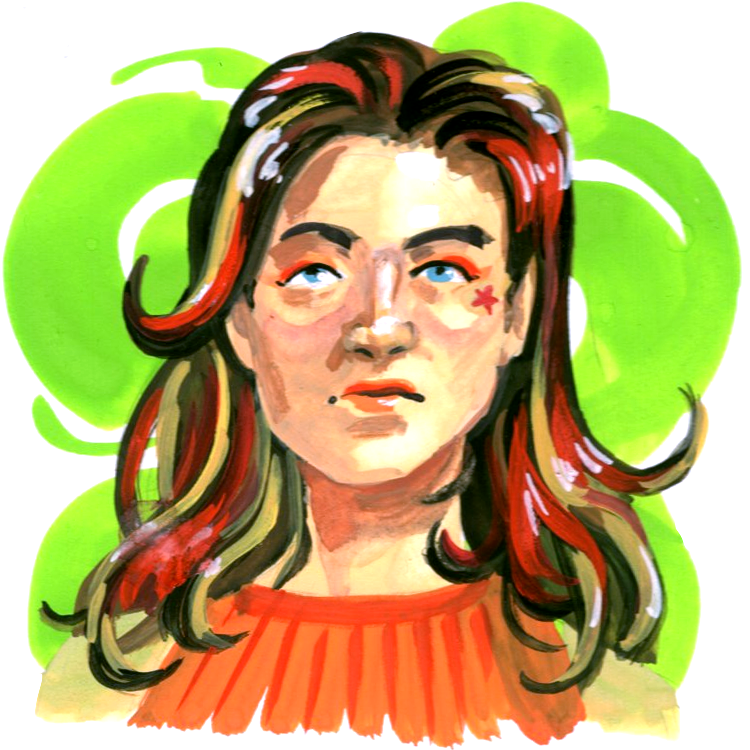
\includegraphics[scale=0.4]{portraits/Flohmarkt_Flash.png}
\end{center}

\newpage
\begin{npcBox}[title=Flash]

    \begin{aspects}
    \item \aspect[High Concept]{Genetics expert shaping the future}
    \item \aspect[Trouble]{At odds with the family she loves}
    \item \aspect[Relationship]{She finds it more normal to have a woman as a father than she herself does.}
    \item \aspect[Aspect]{E-bike addict}
    \end{aspects}

    \begin{skills}
    \item \nskill{Academics}{3}
    \item \nskill{Athletics}{1}
    \item \nskill{Burglary}{0}
    \item \nskill{Contacts}{0}
    \item \nskill{Crafts}{3}
    \item \nskill{Deceive}{1}
    \item \nskill{Drive}{1}
    \item \nskill{Empathy}{0}
    \item \nskill{Fight}{0}
    \item \nskill{Investigate}{2}
    \item \nskill{Lore}{2}
    \item \nskill{Notice}{0}
    \item \nskill{Physique}{0}
    \item \nskill{Provoke}{0}
    \item \nskill{Rapport}{1}
    \item \nskill{Resources}{0}
    \item \nskill{Shoot}{0}
    \item \nskill{Stealth}{0}
    \item \nskill{Will}{2}
    \item \nskill{Prototyping}{4}
    \end{skills}

    \begin{stunts}
    \item \stunt{Small stock}{She prefers smalla nd agile vehicles. Gets +2 on driving if her ride is lighter than she is.}
    \end{stunts}

    \begin{stressSection}
    \stressLine{\stress{1}\stress{1}\stress{1}}{\stress{1}\stress{1}\stress{1}\stress{1}}
    \end{stressSection}
    \begin{tabularx}{\textwidth}{ XX }
    \end{tabularx}

    \begin{consequences}
    \item \consequence{2}
    \item \consequence{4}
    \item \consequence{6}
    \end{consequences}

    \begin{equipment}
    \item An e-bike that is tuned beyond all reason
    \item A genetic engineering kit that can be used to make diagnoses and perform simple procedures
    \end{equipment}
\end{npcBox}
\newpage

\chapter{Other groups}

Lost flea markets aim to bring together several Lost groups. However, it is often easy to find slightly confused Pioneers and Norms.

\section{Jones-es}

This is the name of a group that searches the ruins of the lemmings for technology, books and other valuable or interesting items. They offer their latest finds in exchange for medicines and repairs.

\subsection{Random discoveries from the ruins}

\begin{enumerate}
    \item A crate of old and well-preserved wine bottles. And lots of tins of ravioli.
    \item Perry Rhodan Silver Volumes
    \item Private video tapes from the 1990s – what could be on them?
    \item An old map of this region. However, many of the places no longer exist after the disasters. Is an expedition worthwhile?
    \item A child's essay entitled “This is how I imagine the future”. What does it say ? What did become of that child.
    \item A box with old board games.
\end{enumerate}

The most valuable artefacts are those from the old world that the Lost have recovered during their expeditions. The artefacts of the Lemmings. The Lost in particular rely on ancient technology to repair their vehicles and buildings. Books themselves, however, have an almost spiritual value for the Lost, and rare copies are secretly traded at flea markets. Until someone brings them to “Alexandria” to gain fame, where they are copied and reproduced

Incidentally, Lost people trade in barter, Norms pay with digital money, and among Pioneers, many transactions take place based on the reputation and fame of the individuals involved. At a Lost flea market, culture shock and chaotic chains of barter are therefore inevitable, especially for non-Lost people.

\section{Farmer}

Looking for animals for breeding and plant seeds. They are willing to pay in kind. Spontaneous slaughtering for festive roasts is also to be expected. The large number of animals can cause a manure disposal problem and a terrible stench if this is not planned for in advance.

\section{Craftspeople}

They offer repairs, but they need raw materials.

\section{The fair}

Of course, there are hundreds more people from other groups who cook, repair, sell, buy, read aloud, play music, search and run a fair with all kinds of stalls and attractions. Popular with children: betting on a mouse in a maze: which exit will it take?


